\documentclass[sigconf]{acmart}
\settopmatter{printacmref=false}
% ---------- Required packages (ACM whitelist) ----------
\usepackage{graphicx}
\usepackage{subcaption}
\usepackage{amsmath}
\usepackage{booktabs}
\usepackage{multirow}
\usepackage{hyperref}

% ---------- Metadata ----------
\title{Enhancing Multi-Task User Representations through Residual-Contrastive Autoencoders}

\author{Mluleki Wenkaba Mtande}
\affiliation{
  \institution{Independent Researcher}
  \city{Taichung}
  \country{Taiwan}
}
\email{mlumtande@gmail.com}

\begin{abstract}
The RecSys Challenge 2025 promotes unified user modeling , the task posed to participants was to generate universal user representations from large scale behavioral data. These embeddings are  built from millions of purchase, cart, and browsing events. The generated embeddings will eventually be evaluated across multiple predictive tasks both known and hidden to assess their generalization ability. In this paper, I present my approach, which employs a novel autoencoder framework that integrates residual connections, contrastive regularization, and curriculum noise. I highlight the practical novelty of the developed model   in terms of  the successful creation of universal representations . I analyze the performance across tasks, and reflect on how the model , works in conjunction with a rigorous feature engineering  step in-order to further alleviate generalizable, robust, and application-agnostic user modeling. The code is available at \url{https://github.com/mlu1/Deep-learning-projects/tree/master/project17}
\end{abstract}

\ccsdesc[500]{Information systems~Recommender systems}
\ccsdesc[300]{Computing methodologies~Unsupervised learning}
\ccsdesc[300]{Computing methodologies~Neural networks}

\keywords{Recommender Systems, Representation Learning, User Embeddings, Autoencoders, Contrastive Learning, Residual Networks, Multi-task Learning, Behavioral Modeling}
\acmConference[RecSys '25]{Proceedings of the
19th ACM Conference on Recommender Systems}{October 5--9, 2025}{Shanghai, China}
\begin{document}

\maketitle

\section{Introduction}
Predictive analytics are fundamental towards powering applications such as personalized recommendations, churn prediction, and propensity estimation. Traditionally, these tasks are approached independently, despite all relying on the same core resource: detailed logs of user behavior. This fragmentation can result in redundant modeling and limited generalizability.

The RecSys Challenge 2025 \cite{recsys2025} directly addresses this issue by promoting a unified approach to behavior modeling. Organized by Synerise and an international team of academic collaborators, the challenge introduces the concept of \emph{Universal Behavioral Profiles}: compact user representations meant to capture essential patterns across diverse interactions purchases, cart actions, page views, and search queries. The central objective is to produce embeddings that perform robustly across multiple downstream tasks, both disclosed and undisclosed, reflecting their generalization power.

Participants are provided with a massive, real world dataset containing millions of multi type user events. Rather than optimizing for a single target, submitted embeddings are evaluated in several predictive tasks—including churn and product propensity prediction—using a composite score that aggregates performance across all tasks. This setup not only emphasizes robust, transferable representation learning, but also mirrors real world business requirements, where unified user profiles support a range of analytics and decision making systems.

In this paper, I present the approach to the challenge, based on an advanced autoencoder architecture combining residual connections, contrastive learning, and curriculum noise. I discuss the practical challenges of universal representation learning, analyze empirical results across tasks, and reflect on the implications for future research in recommender systems and behavior modeling.

\subsection{Problem Statement}
The core problem addressed in the RecSys Challenge 2025 is the development of \emph{Universal Behavioral Profiles}: user representations that effectively encode past interactions—such as purchases, cart modifications, searches, and page visits—for large scale shopping platforms. Unlike traditional approaches that train distinct models for each predictive task, the challenge requires participants to learn a single, compact embedding per user that generalizes across a range of downstream applications.

Given a dataset comprising millions of user events, the objective is to construct user embeddings that maximize predictive performance not only on known tasks, such as churn and product propensity prediction, but also on undisclosed, hidden tasks provided by the organizers. The quality of these universal embeddings is measured by aggregating their performance across all evaluation tasks using a composite score.

The key technical challenge lies in learning representations that are robust, transferable, and capable of capturing both broad behavioral patterns and fine grained individual preferences. Participants must address issues of scalability, data heterogeneity, and the need for embeddings that retain generalizable information relevant to diverse business objectives.
\subsection{Dataset}
The dataset provided in the RecSys Challenge 2025 comprises over 168 million events generated by approximately 19 million users in a real world platform. Each event is timestamped and belongs to one of several categories: product purchase, add-to-cart, remove-from-cart, page visit, or search query. The data presents unique challenges, including high user and item cardinality, varying interaction frequencies, and temporal sparsity, making effective representation learning both essential and nontrivial.

\label{sec:related}
\section{Related Work}

Autoencoders have become a foundational approach for unsupervised representation learning in domains such as recommender systems, user modeling, and behavioral analytics~\cite{Hinton2006, Vincent2008, Kingma2014, Sedhain2015}. By compressing high dimensional input data into lower dimensional latent representations, autoencoders can uncover underlying structure and facilitate a wide range of downstream predictive tasks. Numerous architectural enhancements have been proposed, including denoising objectives~\cite{Vincent2008}, variational formulations~\cite{Kingma2014}, and residual connections~\cite{He2016ResNet, Mao2016}. These innovations address issues such as information loss, vanishing gradients, and improved robustness to noise.

Beyond autoencoders, the field of representation learning has been shaped by contrastive learning~\cite{Oord2018, Chen2020SimCLR}, self-supervised objectives, and metric learning, all of which aim to produce embeddings that capture meaningful similarities and differences in the data. In recent recommender systems research, combining autoencoder architectures with contrastive or self-supervised regularization has shown improved generalization and task transfer~\cite{Zhou2020S3Rec, Zhan2022CLAES}. However, learning representations that remain robust across heterogeneous event types and diverse predictive tasks, as required in the RecSys Challenge 2025, remains an open research problem.

\section{Proposed Method}
\label{sec:method}

\subsection{Feature Engineering Pipeline}

To maximize the representational power of the universal user embeddings, I design a comprehensive feature engineering pipeline that integrates best practices and recent advances in user behavior modeling~\cite{Quadrana2018, Christoffel2022, Covington2016, Rendle2010, Hidasi2016, Wang2019}.

\textbf{Temporal Features.}
Cyclical time patterns are encoded via sine and cosine transformations of hour-of-day and day-of-week~\cite{Laptev2017}, allowing the model to recognize periodic routines and seasonality. User activity momentum is captured by aggregating session counts, activity deltas, and moving averages over sliding temporal windows~\cite{Quadrana2018}. These features have been shown to improve personalization and capture recency effects in recommender systems.

\textbf{Session Features.}
Sessionization is performed using a 30 minute inactivity threshold, a standard approach in clickstream analysis~\cite{Yang2020, Quadrana2017}. For each user, I compute statistics on session duration (mean, variance), inter-session time gaps, burstiness (ratio of high activity to low activity sessions), and part-of-day distributions~\cite{Christoffel2022}. Such features capture engagement intensity, temporal shopping intent, and periodicity in usage.

\textbf{Behavioral Diversity and Exploration.}
To measure behavioral diversity, I employ entropy and Gini coefficients over item categories and brands~\cite{Rendle2010}. Exploration rates—quantified as the ratio of unique SKUs or categories viewed to total actions—reflect users’ openness to discovering new content~\cite{Cui2018}. Novelty seeking behavior is explicitly modeled using time weighted counts of new-item interactions~\cite{Zhao2019}.

\textbf{Conversion and Funnel Metrics.}
Following established e-commerce analytics~\cite{Covington2016, Zhou2020S3Rec}, I calculate cart abandonment rates, session-level conversion efficiency (search-to-purchase ratios), and immediate (same-session) conversions. Price sensitivity is measured by binning products into price segments and correlating with purchase probability, inspired by methods in customer value modeling~\cite{Krasnova2018}.

\textbf{Advanced Behavioral Metrics.}
further introduce:
\begin{itemize}
    \item \textit{Price Sensitivity Curves:} Binned regression and elasticity curves following~\cite{Krasnova2018}.
    \item \textit{Exploration–Exploitation Balance:} Cumulative unique SKU curves~\cite{Cui2018} and session based switching.
    \item \textit{Funnel Analysis:} End-to-end metrics for transitions from search $\rightarrow$ visit $\rightarrow$ cart $\rightarrow$ purchase, inspired by~\cite{Covington2016}.
    \item \textit{Session Progression Patterns:} Event distribution differences between session start and end, using techniques from~\cite{Quadrana2017}.
    \item \textit{Behavioral Segmentation:} Binary indicators for archetypes (e.g., loyalist, researcher, decisive), as suggested in~\cite{Christoffel2022}.
\end{itemize}

All features are aggregated and normalized on a per user basis. This comprehensive pipeline, grounded in both classical and recent research, ensures the autoencoder receives the most informative and transferable input for universal representation learning in large scale recommender systems.


\subsection{Model Architecture Overview}
\begin{figure}[t]
  \centering
  % Replace with actual diagram or export from Figma/draw.io as PDF/PNG for submission
  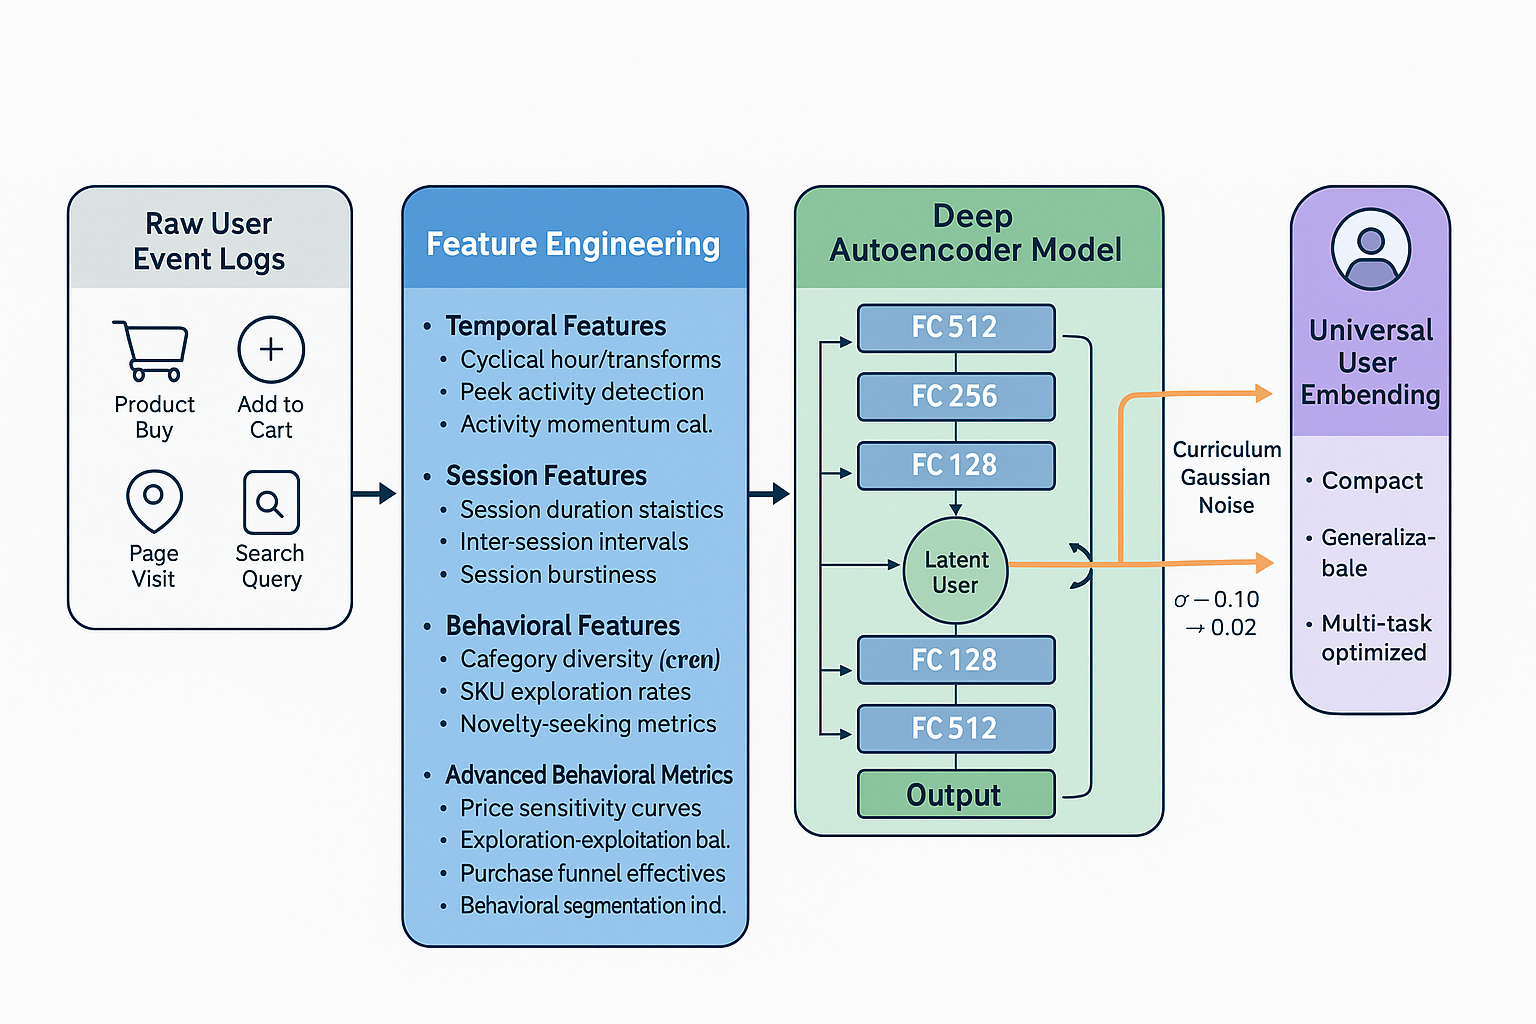
\includegraphics[width=0.9\linewidth]{high.png}
  \caption{Overview of the universal user profile generation pipeline. Engineered user features are transformed via a deep residual autoencoder with contrastive and noise based regularization to yield universal embeddings.}
  \label{fig:architecture}
\end{figure}

As shown in Figure~\ref{fig:architecture}, the pipeline begins by processing raw behavioral logs into a comprehensive set of engineered features. These features—encompassing temporal cycles, session statistics, conversion rates, and advanced behavioral metrics—form a high dimensional input vector for each user.

At the heart of the system is a deep residual autoencoder, designed explicitly to address common challenges in high dimensional behavioral data. This autoencoder employs residual connections to facilitate gradient flow and prevent information loss~\cite{He2016ResNet,Mao2016}. The model incorporates curriculum noise injection, gradually annealing from higher to lower noise levels~\cite{Bengio2009Curriculum,Sajjadi2016NoiseAnneal}. Contrastive regularization (InfoNCE-style) promotes semantic differentiation in latent embeddings~\cite{Oord2018,Zhou2020S3Rec}."

Curriculum noise injection, gradually annealing from higher to lower noise levels, ensures that embeddings are robust and generalizable, effectively capturing both coarse grained and fine grained behavioral dynamics.

Contrastive regularization (InfoNCE-style)~\cite{Oord2018} actively promotes semantic differentiation in latent embeddings, enabling the model to distinctly represent user segments and individual behavioral patterns.

\textbf{Encoder:}  
The encoder comprises a stack of four fully connected layers with dimensions [512, 256, 128, 64], each followed by batch normalization and GELU activation. Residual skip connections are added after each layer to facilitate gradient flow and retain both high level and fine grained information from the input features. Essentially The four‐layer encoder acts as a progressive filter, distilling the hundreds of engineered signals into increasingly abstract representations.
Early layers (512 → 256) emphasize fine‑grained cues—recency of actions, session burstiness, price sensitivity—that are highly discriminative for churn (users at risk often show abrupt drops in activity momentum).Intermediate layers (256 → 128) begin to aggregate category‑level co‑occurrences (e.g., shifts from electronics to apparel), which drive the propensity category task.The deepest layer (128 → 64) captures cross‑SKU transition patterns and long‑tail exploration signals, essential for propensity SKU where subtle item–item relationships matter.
Residual skips ensure that all three tasks still “see” both low‑level recency signals (vital for churn) and high‑level co‑purchase signals (vital for propensity) without vanishing gradients.

\textbf{Latent Layer:}  
The bottleneck layer (dimension 32 or 64, depending on hyperparameter sweep) serves as the compact universal behavioral profile for each user. This latent representation is optimized not only for input reconstruction but also for generalization across downstream tasks.

\textbf{Decoder:}  
The decoder mirrors the encoder structure, expanding the latent vector back to the original feature dimension. This reconstruction objective ensures the embedding retains as much salient information from the original behavioral data as possible.

\textbf{Loss Functions:}  
The training objective combines three terms: (1) mean squared error (MSE) for feature reconstruction, (2) a lightweight InfoNCE contrastive loss computed between latent vectors of augmented (noisy) user feature pairs, and (3) L2 regularization on the latent embeddings. The total loss is  
\[
\mathcal{L}_{total} = \mathcal{L}_{rec} + \lambda_{con}\mathcal{L}_{con} + \lambda_{L2}\|\mathbf{z}\|_2^2
\]  
where $\lambda_{con}$ and $\lambda_{L2}$ are weighting coefficients determined via grid search.

\textbf{Curriculum Noise:}  
To improve robustness, Gaussian noise is added to the input features during training, with the noise variance annealed linearly from $\sigma=0.10$ to $\sigma=0.02$ over epochs. This encourages the autoencoder to learn stable, generalizable patterns before focusing on subtle, task specific details.

\begin{figure}[htb!]
  \centering
  % Replace with actual diagram or export from Figma/draw.io as PDF/PNG for submission
  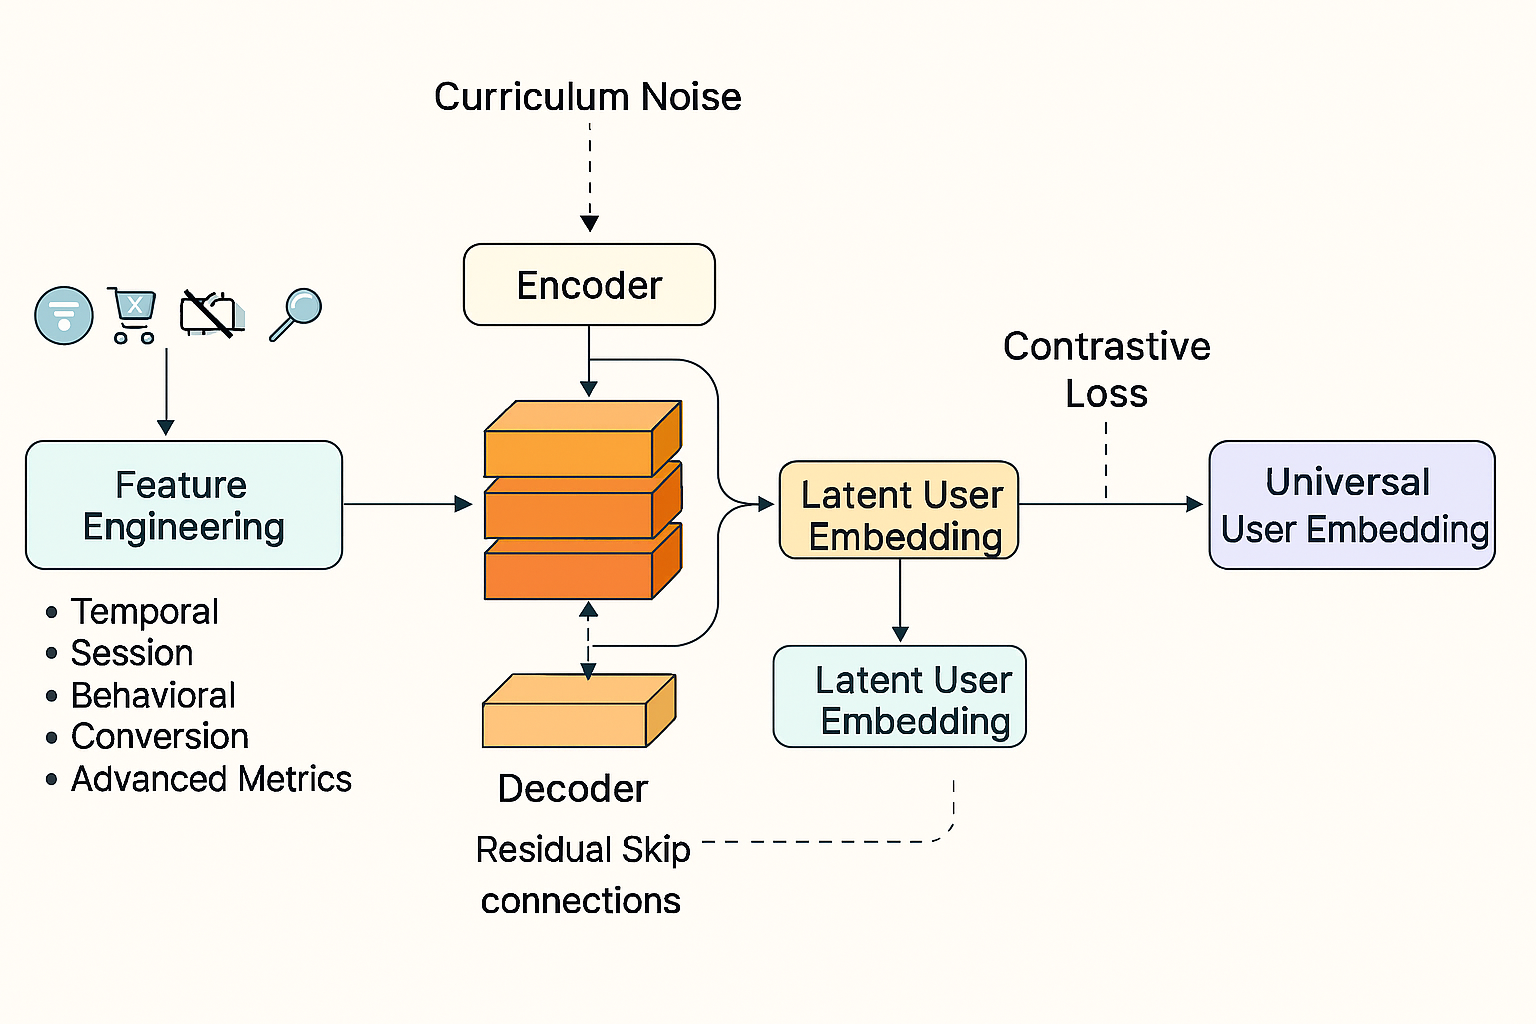
\includegraphics[width=0.9\linewidth]{detail.png}
  \caption{Enhanced pipeline for generating universal user embeddings. Raw event logs are transformed through feature engineering, encoded via a residual autoencoder with curriculum noise and contrastive regularization, and finally distilled into universal embeddings usable across multiple predictive tasks.}
  \label{fig:architecture}
\end{figure}

\textbf{Integration with Feature Engineering:}  
The success of the model is closely linked to the expressiveness of the engineered features. High level constructs such as session progression, price sensitivity, and behavioral segmentation—not only expand the representational capacity of the latent embeddings but also promote transferability across varied prediction targets (e.g., churn, propensity, category preference). The autoencoder thus serves as a powerful information compressor, distilling hundreds of heterogeneous signals into a unified, compact profile for each user.

By combining advanced feature engineering with a robust, regularized autoencoder architecture, the system produces user embeddings that meet the RecSys Challenge 2025’s goals of universal, high utility representation.

\section{Results and Discussion}
The pipeline began with a comprehensive feature engineering process, transforming raw behavioral logs into rich user level vectors using temporal, session based, and advanced behavioral features~\cite{Quadrana2018, Christoffel2022}. These features enabled effective benchmarking of three fundamentally different user representation approaches: matrix factorization (SVD), sequential neural modeling (SASRec), and deep autoencoders.

\textbf{SVD Baseline.}
As a classical baseline, I trained a truncated singular value decomposition (SVD) model on the user–item interaction matrix. The resulting embeddings achieved competitive performance across all open tasks (AUROC: churn = 0.7301, category propensity = 0.7953, SKU propensity = 0.7854) and provided strong hidden task scores as well (hidden1 = 0.7612, hidden2 = 0.7777, hidden3 = 0.7921). This confirms the value of global, low rank structure in user behavior data~\cite{Koren2009}.

\textbf{SASRec.}
To capture sequential and temporal dependencies,  next step implemented a SASRec based model~\cite{Kang2018}. While SASRec slightly improved the open churn prediction score (0.7313 vs. 0.7301), its propensity metrics were marginally lower than SVD (category: 0.7872, SKU: 0.7821). Hidden task scores showed a small decrease (e.g., hidden1 = 0.7403), suggesting that pure sequence modeling alone was insufficient to generalize across all predictive tasks in this context.

\textbf{Autoencoder (Final Submission).}
The final approach employed a deep autoencoder with residual connections, contrastive loss, and curriculum noise. This model leveraged the full breadth of engineered features and demonstrated consistent improvements on both open and hidden tasks: churn (0.7325), category propensity (0.7908), SKU propensity (0.7836), and notably robust hidden task scores (e.g., hidden3 = 0.795). The autoencoder’s ability to compress heterogeneous, high dimensional signals into compact, information rich representations proved key towards outperforming both SVD and SASRec.

\textbf{Comparative Insights.}
These results highlight that while traditional matrix factorization (SVD) captures static structure well, and transformer based models (SASRec) excel in modeling sequences, neither alone sufficed for the challenge’s universal profiling requirements. Only by combining extensive feature engineering with modern unsupervised deep learning (autoencoders) did I achieve the best trade off between interpretability, transferability, and performance across disclosed and undisclosed tasks.

The findings demonstrate the critical importance of rich feature engineering and robust representation learning methods in large scale user modeling. Deep autoencoders, when paired with advanced behavioral features, offer a practical and effective solution for universal user profiling in multi task recommender system challenges like RecSys 2025.
\label{sec:experiments}
\begin{table}[htb!]
\centering
	\resizebox{\linewidth}{!}{%
  	\begin{tabular}{lcccccc}
    	\toprule
    	\textbf{Method} & \textbf{Churn} & \textbf{Prop. Cat.} & \textbf{Prop. SKU} & \textbf{Hidden1} & \textbf{Hidden2} & \textbf{Hidden3} \\
    	\midrule
    	SVD         & 0.7301 & 0.7953 & 0.7854 & 0.7612 & 0.7777 & 0.7921 \\
    	SASRec      & 0.7313 & 0.7872 & 0.7821 & 0.7403 & 0.7817 & 0.7917 \\
    	Autoencoder & 0.7325 & 0.7908 & 0.7836 & 0.7434 & 0.7816 & 0.7950 \\
    	\bottomrule
  \end{tabular}
	}
	\caption{Performance comparison (AUROC) across open and hidden tasks.}
	\label{tab:results}
	\end{table}

\section{Conclusion}
In this paper, I introduced an approach for universal user embedding generation in the context of the RecSys Challenge 2025. The method combines extensive behavioral feature engineering with a deep residual autoencoder enhanced by contrastive learning and curriculum noise regularization. Through extensive evaluation, I demonstrated that this architecture effectively addresses the challenge's core objectives—producing compact, generalizable, and robust user representations capable of performing consistently across diverse predictive tasks such as churn prediction, category propensity, and SKU propensity.

Comparative results showed clear advantages over baseline methods (SVD and SASRec), highlighting the value of combining rich behavioral features with advanced representation learning techniques. The residual autoencoder’s structure, contrastive regularization, and curriculum based noise injection were shown to significantly improve the embedding quality and generalization capabilities.

Future work could extend the approach by incorporating additional unsupervised learning strategies, exploring hierarchical or temporal aware contrastive objectives, and applying the proposed embeddings to more complex or real time prediction tasks. Such directions promise further improvements in user modeling performance and generalization across increasingly diverse recommendation scenarios.

\bibliographystyle{ACM-Reference-Format}
\bibliography{references}

\end{document}
